\chapter{Diagramme de classes}

\section{Diagramme}

\begin{figure}
  \centering
  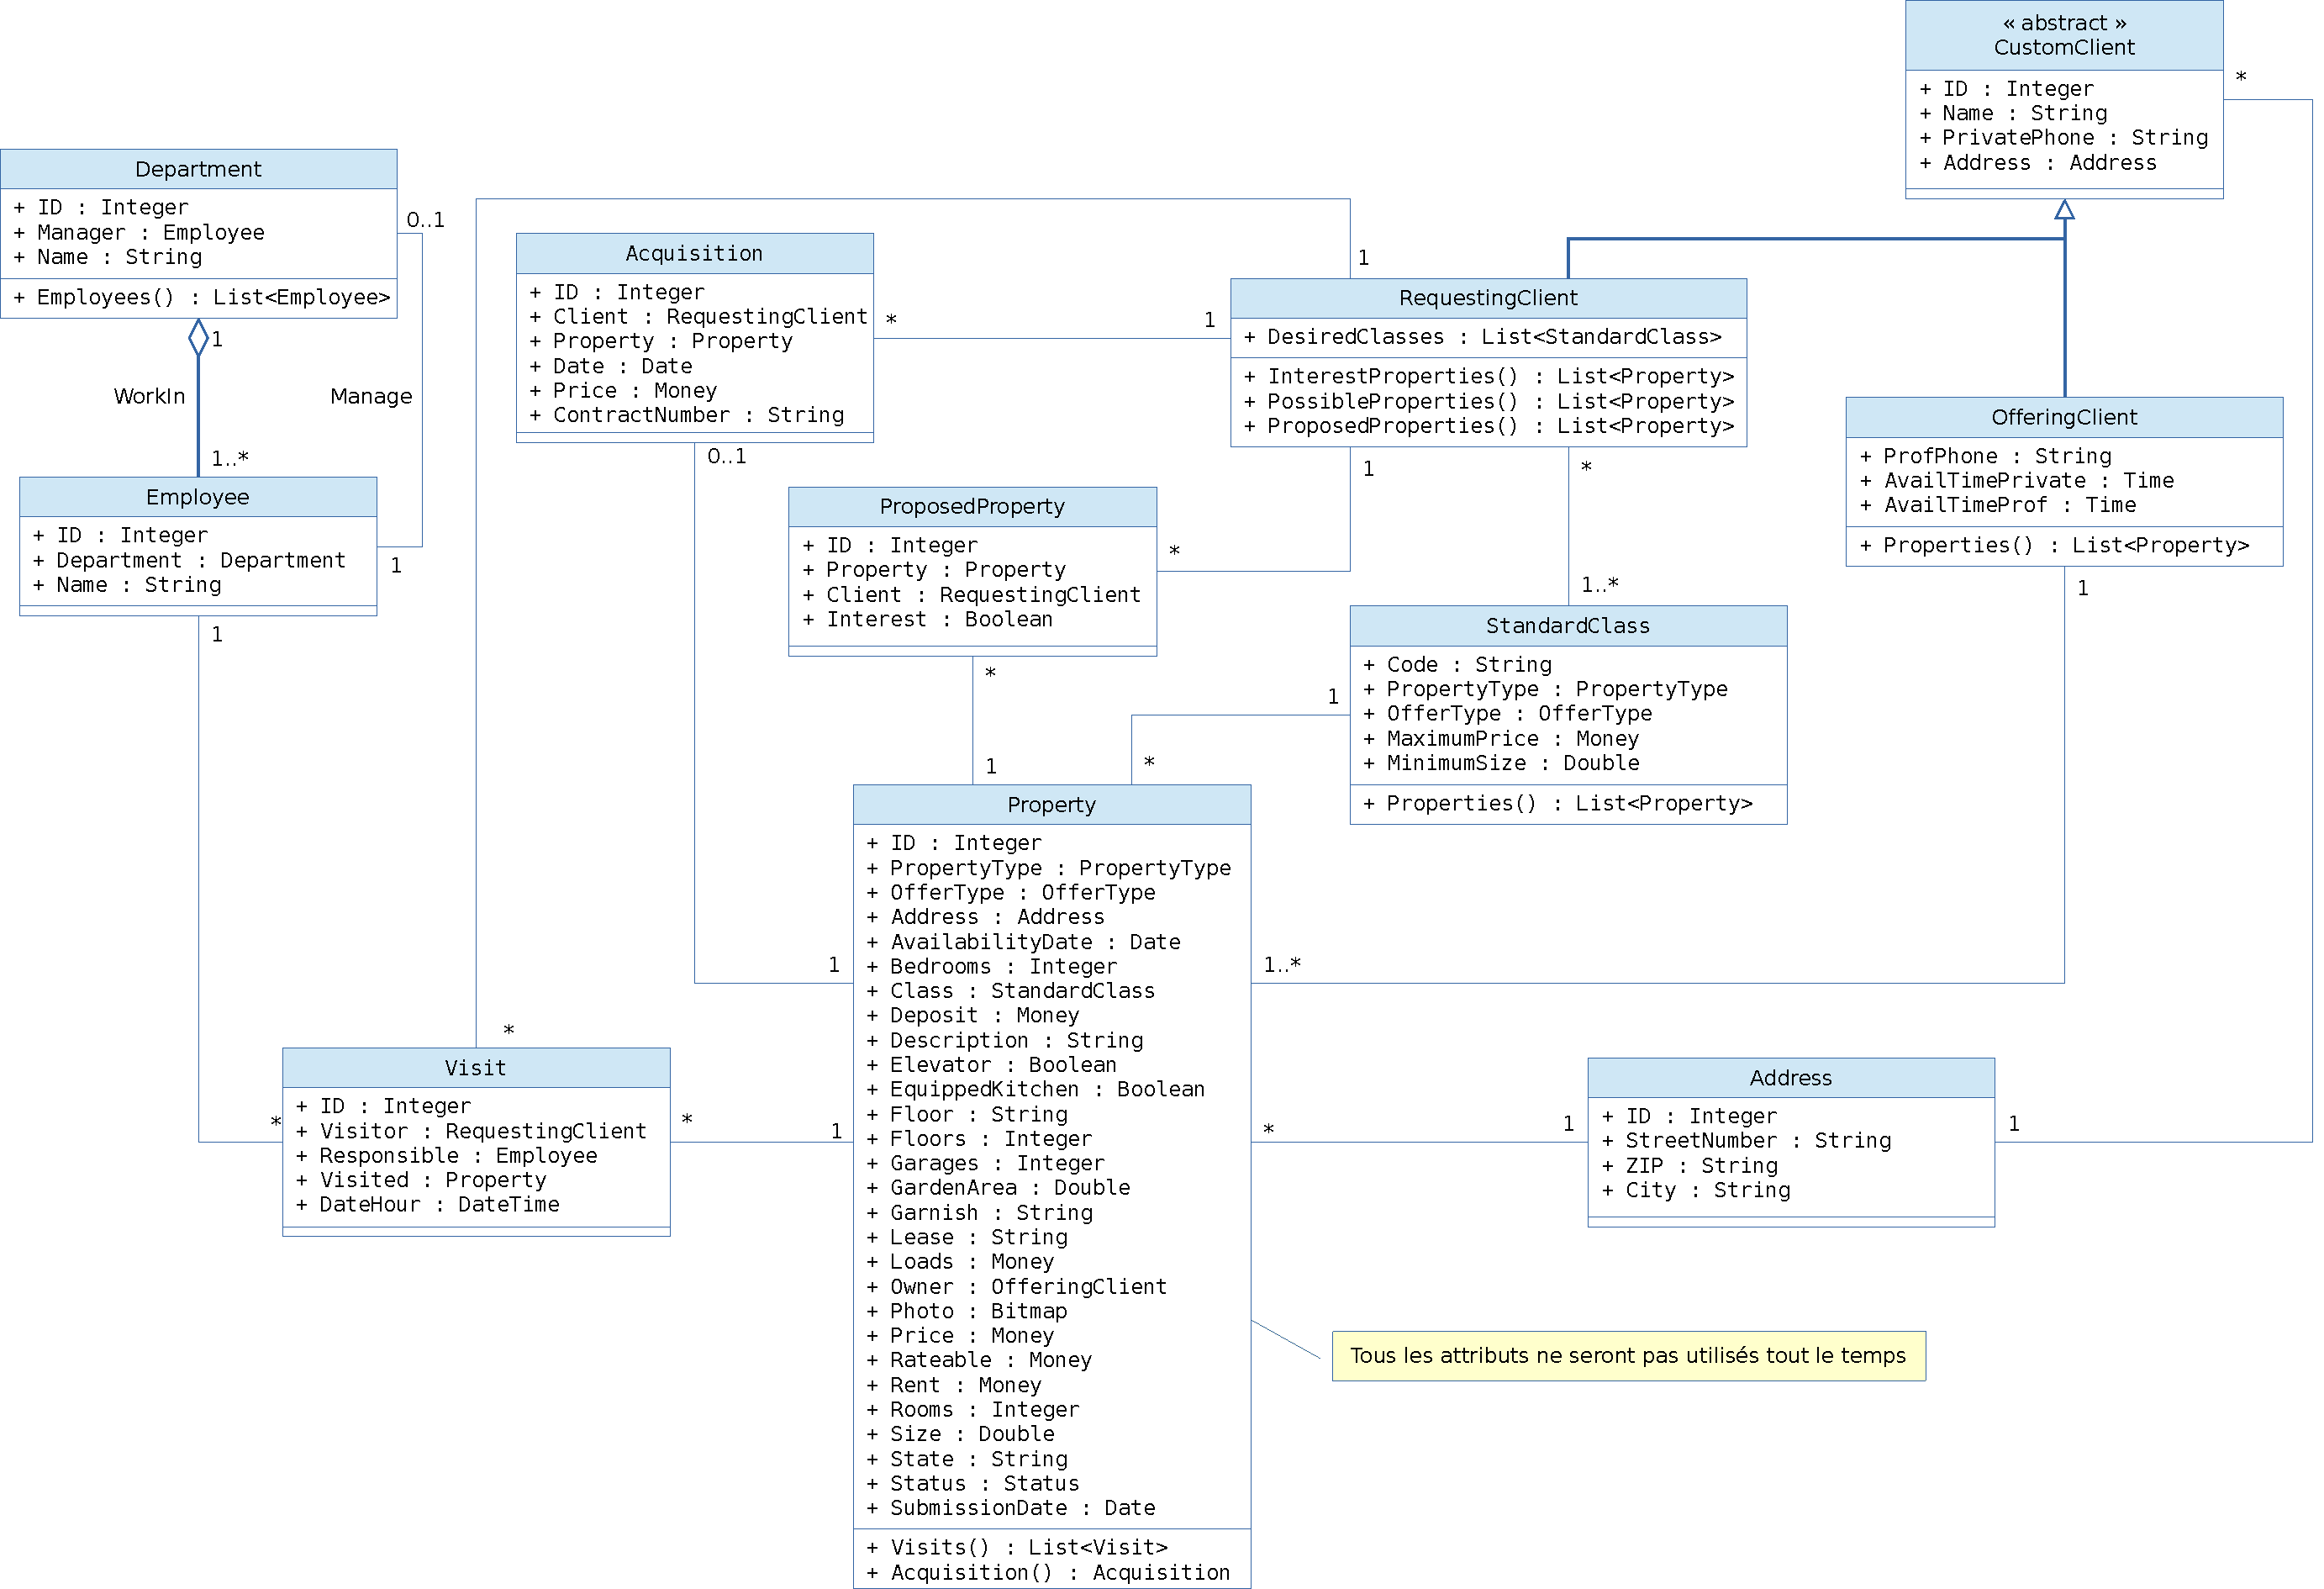
\includegraphics[angle=90,height=0.99\textheight]{IMG/cd}
  \caption{Diagramme de classes}
  \label{img_cd}
\end{figure}

La figure \refpage{img_cd} illustre le diagramme de classes du projet.

\section{Règles métier}

Les règles métier de ce diagrammes figurent dans le tableau \refpage{tbl_business_rules}.

\begin{table}
  \begin{tabular}{|p{0.95\textwidth}|}
  \hline
  \rowcolor{gray05} \multicolumn{1}{|c|}{\textbf{Contraintes}} \\
  \hline
  \hline
  % manager
  \textbf{(BR001)} Le manager d'un département doit appartenir au département. \\
  % responsable visite
  \textbf{(BR002)} Pour pouvoir faire visiter un bien, l'employer doit appartenir au service des visites. \\
  % terrain -> vente uniquement
  \textbf{(BR003)} Un terrain ne pourra pas être mis en location (vente uniquement). \\
  % attributs valides tout le temps
  \textbf{(BR004)} Pour tout bien immobilier, il faudra indiquer son statut (disponible, loué ou acheté), la classe standard à laquelle il appartient,
la date à laquelle le bien lui a été soumis, sa localisation, la date de mise en disposition, le revenu cadastral. \\
  % description
  \textbf{(BR005)} Pour tout bien immobilier sauf terrain, il faudra indiquer une description du contenu en termes de nombre et nature des
pièces, type de chauffage, etc. (texte libre). \\
  % attributs valides pour les locations
  \textbf{(BR006)} Pour tout bien immobilier à louer, il faudra indiquer le montant de la caution locative, le loyer mensuel, le montant mensuel
des charges, le type de bail, la \og{}garniture\fg{} (meublé, non meublé). \\
  % attributs valides pour les ventes
  \textbf{(BR007)} Pour tout bien immobilier à acheter, il faudra indiquer le prix d'achat demandé. \\
  % attributs valides pour les ventes, sauf terrain
  \textbf{(BR008)} Pour tout bien immobilier à acheter, sauf terrain, il faudra indiquer l'état (à restaurer, correct, impeccable). \\
  % attributs valides pour maison et appartement
  \textbf{(BR009)} Pour tout bien de type \og{}maison\fg{} ou \og{}appartement\fg{}, il faudra indiquer le nombre de chambres, le nombre de garages, la présence ou non d'une cuisine équipée, la superficie du jardin éventuel. \\
  % attributs valides pour maison
  \textbf{(BR010)} Pour tout bien de type \og{}maison\fg{}, il faudra indiquer le nombre d'étages. \\
  % attributs valides pour appartement et studio
  \textbf{(BR011)} Pour tout bien de type \og{}appartement\fg{} ou \og{}studio\fg{}, il faudra indiquer l'étage auquel il est localisé et la présence ou non d'ascenseur. \\
  % attributs valides pour terrain
  \textbf{(BR012)} Pour tout bien de type \og{}terrain\fg{}, il faudra indiquer sa superficie. \\
  % attributs valides pour emplacement pour bureaux ou commerce
  \textbf{(BR013)} Pour tout bien de type \og{}emplacement pour bureaux ou commerce\fg{}, il faudra indiquer sa superficie et le nombre de pièces le composant. \\
  \hline
  \end{tabular}
  \caption{Règles métier du diagramme de classes}
  \label{tbl_business_rules}
\end{table}

\section{Rapport}

J'ai réalisé ce diagramme en troisième lieu. Il est basé sur le diagramme entités-associations et représente la structure des différentes données qui seront implémentées. Nous nous sommes ici plus proche de la réalité que du conceptuel.

%Vu la complexité des biens immobiliers, j'ai décidé de mettre tous les attributs possibles à l'entité \og{}Bien immobilier\fg{}. Suivant la valeur des attributs \og{}Type bien\fg{} et \og{}Type offre\fg{}, les attributs auront une valeur pertinente ou non. La table \refpage{tbl_usage_attribut_bien_immobilier} nous donne les conditions de validité des attributs.

%J'ai défini une entité \og{}Adresse\fg{} qui sera associée aussi bien aux clients qu'au biens immobiliers. En effet, le concept de localisation des biens immobiliers est identique à celui de localisation des clients.

%J'ai défini une entité générique pour les client. Ensuite j'ai créé des entités plus spécialisées pour les clients offrants et les clients cherchant un bien. À mon sens, un client qui aujourd'hui est un client cherchant un bien peut demain être un client offrant un bien, d'où l'utilisation d'un client générique. L'entité \og{}Client\fg{} n'offre actuellement pas d'attributs supplémentaires par rapport au client générique. J'ai quand-même créé une entité spécialisée pour permettre une éventuelle évolution future.